%!TEX program = xelatex

\documentclass[compress]{beamer}
%--------------------------------------------------------------------------
% Common packages
%--------------------------------------------------------------------------
\usepackage[english]{babel}
\usepackage{pgfpages} % required for notes on second screen
\usepackage{graphicx}

\usepackage{multicol}

\usepackage{tabularx,ragged2e}
\usepackage{booktabs}


\usetheme{hri}

\usepackage{tikz}
\usetikzlibrary{mindmap,backgrounds,positioning}

\graphicspath{{figs/}}

%--------------------------------------------------------------------------
% General presentation settings
%--------------------------------------------------------------------------
\title{RGB-D Cameras for Human-Robot Interaction}
\subtitle{...}
\date{\today}
\author{Séverin Lemaignan}
\institute{Centre for Neural Systems and Robotics\\{\Medium Plymouth University}}

%--------------------------------------------------------------------------
% Notes settings
%--------------------------------------------------------------------------
%\setbeameroption{show notes on second screen}

\begin{document}
%--------------------------------------------------------------------------
% Titlepage
%--------------------------------------------------------------------------

\maketitle

\section*{Overview}
\begin{frame}{Overview}
    \tableofcontents[hideallsubsections]
\end{frame}


%%%%%%%%%%%%%%%%%%%%%%%%%%%%%%%%%%%%%%%%%%%%%%%%%%%%%%%%%%%%%%%%%%%%%%%
%%%%%%%%%%%%%%%%%%%%%%%%%%%%%%%%%%%%%%%%%%%%%%%%%%%%%%%%%%%%%%%%%%%%%%%
%%%%%%%%%%%%%%%%%%%%%%%%%%%%%%%%%%%%%%%%%%%%%%%%%%%%%%%%%%%%%%%%%%%%%%%

\section{3D Perception for HRI}

\imageframe{pr2-baby-3.jpg}

\begin{frame}{Situation Assessment}
        \centering
        \video{0.7\textwidth}{videos/model3d.webm?autostart&start=22}\\
        \vspace*{1em}
        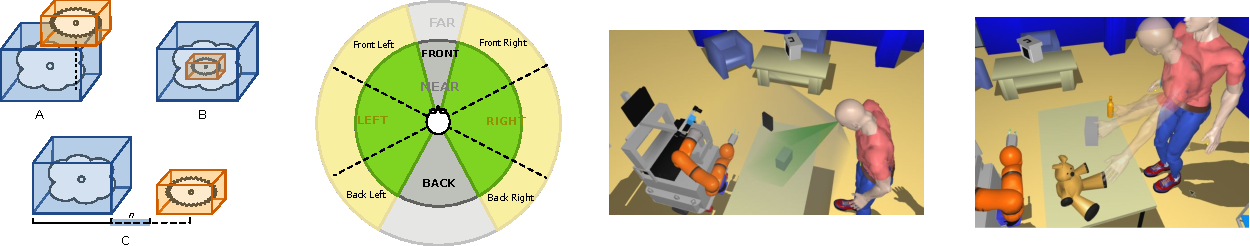
\includegraphics[width=0.9\textwidth]{spark.pdf}
\end{frame}

\begin{frame}{Why not 2D?}
    3D interpretation of a 2D scene is hard!

    Resorts to fiducial markers
\end{frame}

\begin{frame}{Perceiving the humans}

Previously,...

\begin{itemize}
    \item face detection
    \item blob detection
    \item motion capture (+10K pounds)
\end{itemize}

And then, one morning... PrimeSense Kinect! (~150 pounds)

\end{frame}


%%%%%%%%%%%%%%%%%%%%%%%%%%%%%%%%%%%%%%%%%%%%%%%%%%%%%%%%%%%%%%%%%%%%%%%
%%%%%%%%%%%%%%%%%%%%%%%%%%%%%%%%%%%%%%%%%%%%%%%%%%%%%%%%%%%%%%%%%%%%%%%
%%%%%%%%%%%%%%%%%%%%%%%%%%%%%%%%%%%%%%%%%%%%%%%%%%%%%%%%%%%%%%%%%%%%%%%
\section{RGB-D cameras}

\begin{frame}{Perception of depth}
\end{frame}

\begin{frame}{RGB-D cameras: many technologies}
    \begin{itemize}
        \item Stereo-vision
        \item Structured light
        \item Time-of-Flight
    \end{itemize}
\end{frame}

\imageframe{stereo_head}

\begin{frame}{Stereo-vision: principle}
    \begin{multicols}{2}

    \begin{center}
        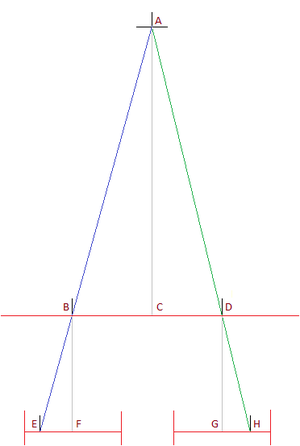
\includegraphics[height=0.8\paperheight]{stereo}
    \end{center}

    \begin{align} 
d &= EF + GH \\ 
    &= BF (\frac{EF}{BF} + \frac{GH}{BF})\\ 
    &= BF (\frac{EF}{BF} + \frac{GH}{DG})  \\ 
    &= BF (\frac{BC + CD}{AC})  \\ 
    &= BF \frac{BD}{AC}  \\ 
    &= \frac{k}{z}  \text{, where} \end{align}
        $k = BD \times BF$\\
        $z = AC$
\end{multicols}
\end{frame}

\begin{frame}{Disparity map}

    \only<1>{
    The disparity map is built by:
    \begin{itemize}
        \item 1) properly aligning the images ({\Medium
    image rectification}), 
        \item 2) looking for the {\Medium disparity} of each pixel between
    the left and right images.
    \end{itemize}
    }

    \only<2>{
        Pixel disparity: for each {\Medium pixel patch} on the left, by how many pixel the
        same patch is {\Medium shifted} on the right?

        \begin{center}
            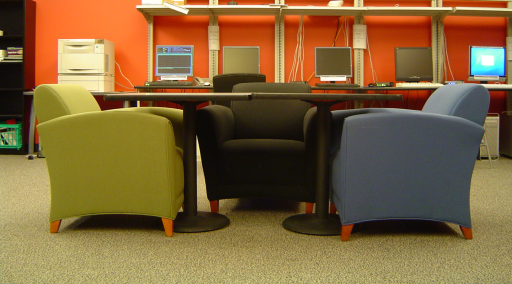
\includegraphics[width=0.45\linewidth]{scene_left}
            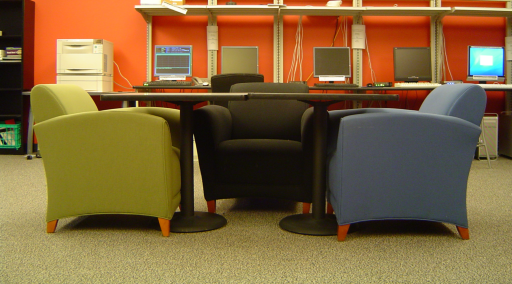
\includegraphics[width=0.45\linewidth]{scene_right}

            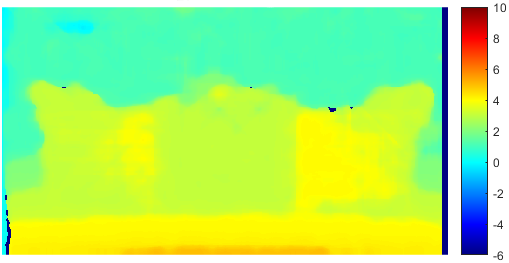
\includegraphics[width=0.45\linewidth]{disparity}
        \end{center}
    }


\end{frame}
\begin{frame}{Issues with stereovision}
    \begin{itemize}
    \item Requires texture $\Rightarrow$ active stereovision
    \item Computation intensive (less of an issue since computations are
        performed on-board)
    \end{itemize}
\end{frame}


\begin{frame}{Active stereo-vision}
    \begin{center}
        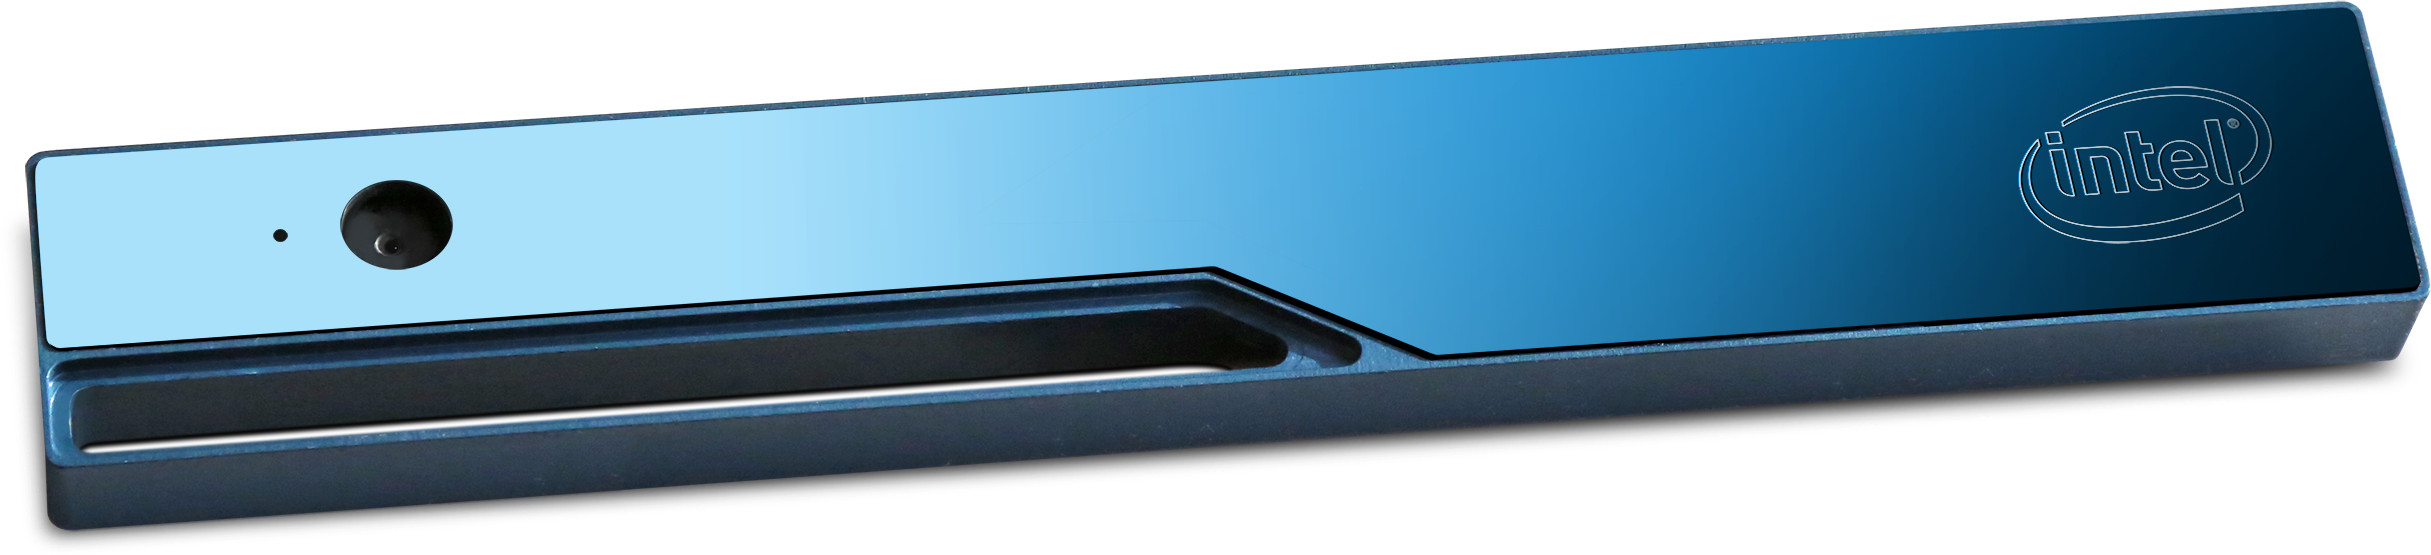
\includegraphics[width=0.8\linewidth]{r200}

        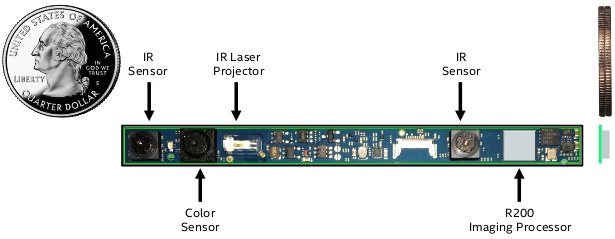
\includegraphics[width=0.8\linewidth]{r200_inside}
    \end{center}
\end{frame}

{
    \paper{Source:
    http://www.hackengineer.com/structured-light-vs-microsoft-kinect/}
    \begin{frame}{Structured light}
        \centering
        \only<1>{
            \video{0.8\linewidth}{videos/structured_light.mp4}
        }
        \only<2>{


            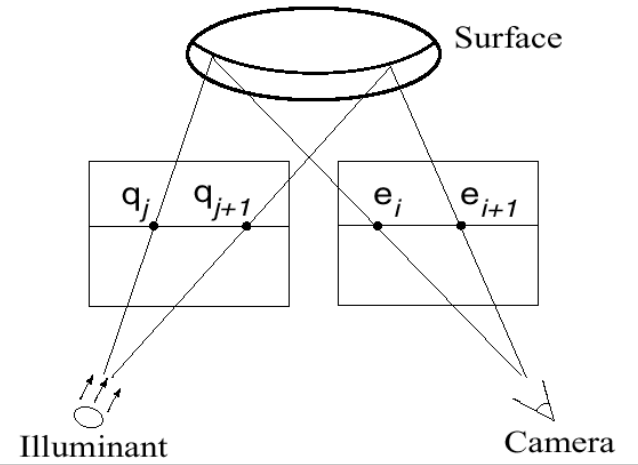
\includegraphics[width=0.8\linewidth]{structured_light_schema}
        }
        \only<3>{

            \video{0.8\linewidth}{videos/structured_light.mp4}

            \begin{table}[htpb]
                \centering
                \begin{tabular}{ccc}
                    & {\Medium Yellow} & {\Medium Red} \\
                    Gray code & 110100111 & 010000111 \\
                    Projector col. & 314 & 250 \\
                    Camera col. & 335 & 392 \\
                    {\Medium Disparity} & 335-314=21 & 392-250=142 \\

                \end{tabular}
            \end{table}
        }

    \end{frame}
}

\begin{frame}{Structured light cameras}
    \begin{center}
        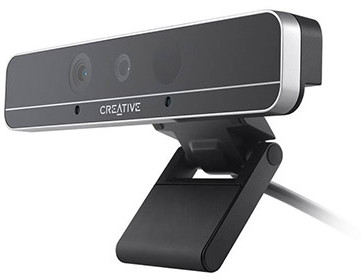
\includegraphics[width=0.4\linewidth]{f200}
        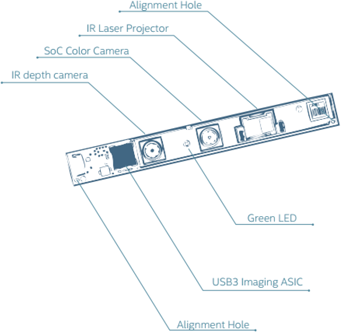
\includegraphics[width=0.6\linewidth]{f200_module}
    \end{center}
\end{frame}


{\fullbackground{kinect360}
\begin{frame}{Speckle decorrelation}


\end{frame}
}

\imageframe[color=black]{kinect_pattern}
\imageframe[color=black]{kinect_pattern2}

\begin{frame}{Structured light}
    \begin{center}
        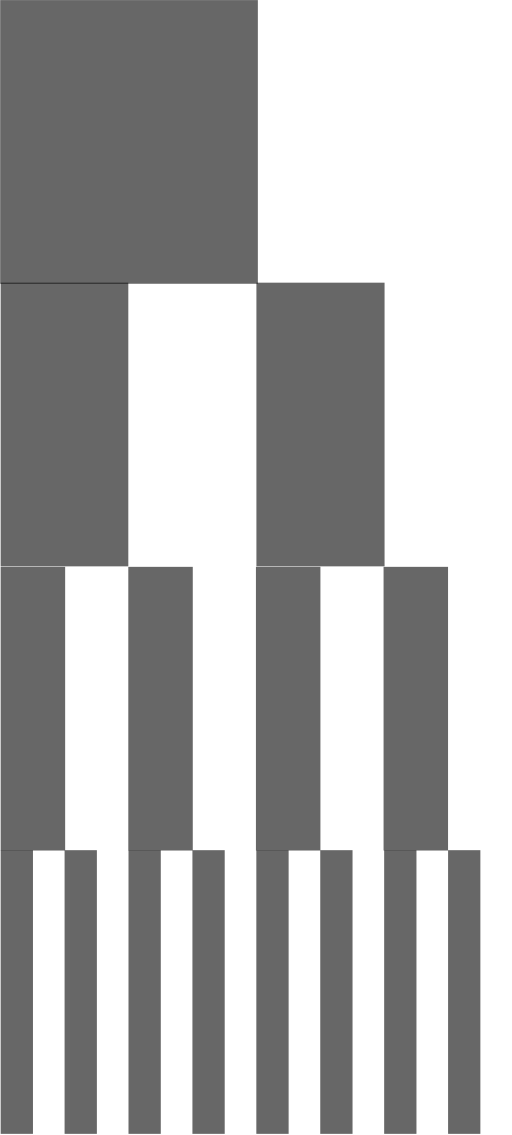
\includegraphics[width=0.8\linewidth]{structured_light}
    \end{center}
\end{frame}

\begin{frame}{Time-of-Flight cameras}
    \begin{center}
        \includegraphics<1>[width=0.8\linewidth]{kinect_xbox_one}
        \includegraphics<2>[width=0.8\linewidth]{tof1}
    \end{center}
\end{frame}


%%%%%%%%%%%%%%%%%%%%%%%%%%%%%%%%%%%%%%%%%%%%%%%%%%%%%%%%%%%%%%%%%%%%%%%
%%%%%%%%%%%%%%%%%%%%%%%%%%%%%%%%%%%%%%%%%%%%%%%%%%%%%%%%%%%%%%%%%%%%%%%
%%%%%%%%%%%%%%%%%%%%%%%%%%%%%%%%%%%%%%%%%%%%%%%%%%%%%%%%%%%%%%%%%%%%%%%

\section{Processing the depth image}

\begin{frame}{RGB-D registration}
\end{frame}

\begin{frame}{Point clouds}
\end{frame}

\begin{frame}{Surface reconstruction}
\end{frame}

\begin{frame}{The typical pipeline}
    Example from ROS?

    One major library: the Point Cloud Library (PCL)
\end{frame}


%%%%%%%%%%%%%%%%%%%%%%%%%%%%%%%%%%%%%%%%%%%%%%%%%%%%%%%%%%%%%%%%%%%%%%%
%%%%%%%%%%%%%%%%%%%%%%%%%%%%%%%%%%%%%%%%%%%%%%%%%%%%%%%%%%%%%%%%%%%%%%%
%%%%%%%%%%%%%%%%%%%%%%%%%%%%%%%%%%%%%%%%%%%%%%%%%%%%%%%%%%%%%%%%%%%%%%%

\section{Algorithms for point clouds}

\begin{frame}{Template matching}
ICP, RANSAC
\end{frame}

\begin{frame}{Point clouds registration}
    \begin{center}
        \includegraphics<1>[width=\linewidth]{scans}
        \includegraphics<2>[width=0.8\linewidth]{registered}
    \end{center}

    \only<3>{
        Registration $\equiv$ estimating the rigid transformation of the imaging
        sensor between scans.
    }
\end{frame}

\begin{frame}{Registration algorithm}

        \begin{center}
            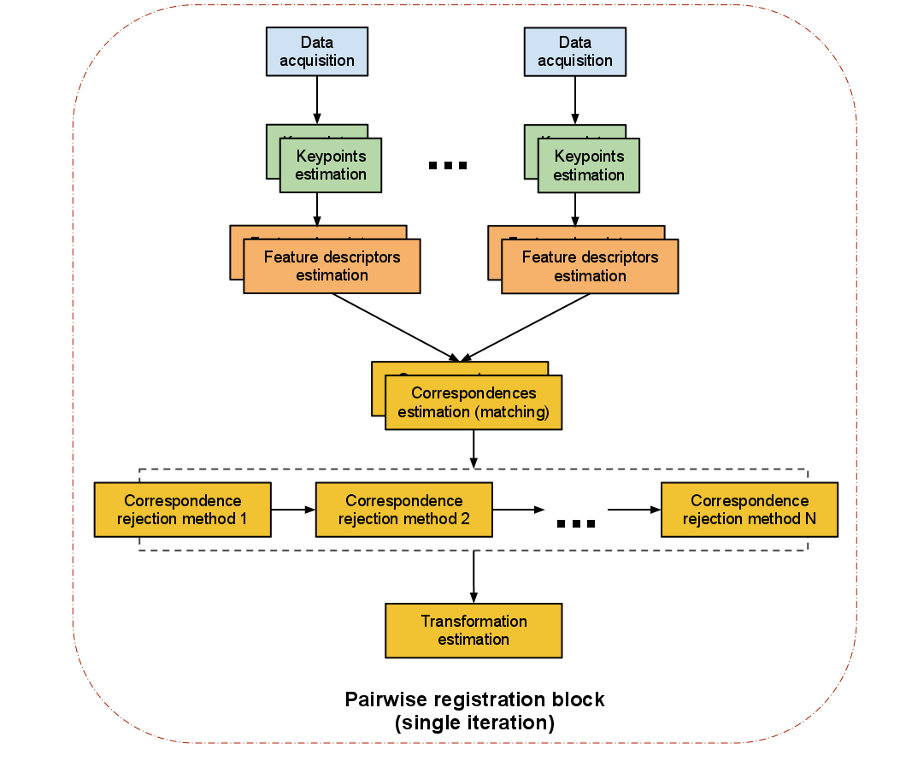
\includegraphics[height=0.8\paperheight]{registration_process}
        \end{center}

        \note{
        Iterative technique.

The computational steps for two datasets are straighforward:

\begin{itemize}
    \item from a set of points, identify **interest points** (i.e., **keypoints**)
        that best represent the scene in both datasets;

    \item at each keypoint, compute a **feature descriptor**;

    \item from the set of **feature descriptors** together with their XYZ
        positions in the two datasets, estimate a set of **correspondences**,
        based on the similarities between features and positions;

    \item  given that the data is assumed to be noisy, not all correspondences
        are valid, so reject those bad correspondences that contribute
        negatively to the registration process;

    \item from the remaining set of good correspondences, estimate a motion
        transformation.

\end{itemize}
    }
\end{frame}

\begin{frame}{Plane segmentation}
\end{frame}

\begin{frame}{Object segmentation}
\end{frame}

\begin{frame}{Octrees}

\end{frame}

\begin{frame}{Skeleton tracking}
\end{frame}


%%%%%%%%%%%%%%%%%%%%%%%%%%%%%%%%%%%%%%%%%%%%%%%%%%%%%%%%%%%%%%%%%%%%%%%
%%%%%%%%%%%%%%%%%%%%%%%%%%%%%%%%%%%%%%%%%%%%%%%%%%%%%%%%%%%%%%%%%%%%%%%
%%%%%%%%%%%%%%%%%%%%%%%%%%%%%%%%%%%%%%%%%%%%%%%%%%%%%%%%%%%%%%%%%%%%%%%

\section{Skeleton Tracking}

\begin{frame}{Skeleton Tracking}
\end{frame}

\begin{frame}{Postures}
\end{frame}

\begin{frame}{Gestures}
\end{frame}

\begin{frame}{Attention}
\end{frame}


%%%%%%%%%%%%%%%%%%%%%%%%%%%%%%%%%%%%%%%%%%%%%%%%%%%%%%%%%%%%%%%%%%%%%%%
%%%%%%%%%%%%%%%%%%%%%%%%%%%%%%%%%%%%%%%%%%%%%%%%%%%%%%%%%%%%%%%%%%%%%%%
%%%%%%%%%%%%%%%%%%%%%%%%%%%%%%%%%%%%%%%%%%%%%%%%%%%%%%%%%%%%%%%%%%%%%%%

\section{One example: greetings recognizer}

\begin{frame}{Recognizing hand waving}
    \begin{itemize}
        \item Acquiring a depth image
        \item Extracting the skeleton
        \item Conversion to joint space
        \item Implementating an HMM
        \item Classifying incoming gestures
    \end{itemize}
\end{frame}


\end{document}






